%%
% Copyright (c) 2017 - 2025, Pascal Wagler;
% Copyright (c) 2014 - 2025, John MacFarlane
%
% All rights reserved.
%
% Redistribution and use in source and binary forms, with or without
% modification, are permitted provided that the following conditions
% are met:
%
% - Redistributions of source code must retain the above copyright
% notice, this list of conditions and the following disclaimer.
%
% - Redistributions in binary form must reproduce the above copyright
% notice, this list of conditions and the following disclaimer in the
% documentation and/or other materials provided with the distribution.
%
% - Neither the name of John MacFarlane nor the names of other
% contributors may be used to endorse or promote products derived
% from this software without specific prior written permission.
%
% THIS SOFTWARE IS PROVIDED BY THE COPYRIGHT HOLDERS AND CONTRIBUTORS
% "AS IS" AND ANY EXPRESS OR IMPLIED WARRANTIES, INCLUDING, BUT NOT
% LIMITED TO, THE IMPLIED WARRANTIES OF MERCHANTABILITY AND FITNESS
% FOR A PARTICULAR PURPOSE ARE DISCLAIMED. IN NO EVENT SHALL THE
% COPYRIGHT OWNER OR CONTRIBUTORS BE LIABLE FOR ANY DIRECT, INDIRECT,
% INCIDENTAL, SPECIAL, EXEMPLARY, OR CONSEQUENTIAL DAMAGES (INCLUDING,
% BUT NOT LIMITED TO, PROCUREMENT OF SUBSTITUTE GOODS OR SERVICES;
% LOSS OF USE, DATA, OR PROFITS; OR BUSINESS INTERRUPTION) HOWEVER
% CAUSED AND ON ANY THEORY OF LIABILITY, WHETHER IN CONTRACT, STRICT
% LIABILITY, OR TORT (INCLUDING NEGLIGENCE OR OTHERWISE) ARISING IN
% ANY WAY OUT OF THE USE OF THIS SOFTWARE, EVEN IF ADVISED OF THE
% POSSIBILITY OF SUCH DAMAGE.
%%

%%
% This is the Eisvogel pandoc LaTeX template.
%
% For usage information and examples visit the official GitHub page:
% https://github.com/Wandmalfarbe/pandoc-latex-template
%%
% Options for packages loaded elsewhere
\PassOptionsToPackage{unicode}{hyperref}
\PassOptionsToPackage{hyphens}{url}
\PassOptionsToPackage{dvipsnames,svgnames,x11names,table}{xcolor}
\documentclass[
  american,
  11pt,
  letterpaper,
  oneside  ,captions=tableheading
]{scrartcl}
\usepackage{xcolor}
\usepackage[margin=1in]{geometry}
\usepackage{amsmath,amssymb}

% add backlinks to footnote references, cf. https://tex.stackexchange.com/questions/302266/make-footnote-clickable-both-ways
\usepackage{footnotebackref}
\setcounter{secnumdepth}{5}
\usepackage{iftex}
\ifPDFTeX
  \usepackage[T1]{fontenc}
  \usepackage[utf8]{inputenc}
  \usepackage{textcomp} % provide euro and other symbols
\else % if luatex or xetex
  \usepackage{unicode-math} % this also loads fontspec
  \defaultfontfeatures{Scale=MatchLowercase}
  \defaultfontfeatures[\rmfamily]{Ligatures=TeX,Scale=1}
\fi
\usepackage{lmodern}
\ifPDFTeX\else
  % xetex/luatex font selection
\fi
% Use upquote if available, for straight quotes in verbatim environments
\IfFileExists{upquote.sty}{\usepackage{upquote}}{}
\IfFileExists{microtype.sty}{% use microtype if available
  \usepackage[]{microtype}
  \UseMicrotypeSet[protrusion]{basicmath} % disable protrusion for tt fonts
}{}

\usepackage{setspace}
\makeatletter
\@ifundefined{KOMAClassName}{% if non-KOMA class
  \IfFileExists{parskip.sty}{%
    \usepackage{parskip}
  }{% else
    \setlength{\parindent}{0pt}
    \setlength{\parskip}{6pt plus 2pt minus 1pt}}
}{% if KOMA class
  \KOMAoptions{parskip=half}}
\makeatother
\usepackage{listings}
\newcommand{\passthrough}[1]{#1}
\lstset{defaultdialect=[5.3]Lua}
\lstset{defaultdialect=[x86masm]Assembler}
\usepackage{etoolbox}
\BeforeBeginEnvironment{lstlisting}{\par\noindent\begin{minipage}{\linewidth}}
\AfterEndEnvironment{lstlisting}{\end{minipage}\par\addvspace{\topskip}}
\usepackage{longtable,booktabs,array}
\newcounter{none} % for unnumbered tables
\usepackage{calc} % for calculating minipage widths
% Correct order of tables after \paragraph or \subparagraph
\usepackage{etoolbox}
\makeatletter
\patchcmd\longtable{\par}{\if@noskipsec\mbox{}\fi\par}{}{}
\makeatother
% Allow footnotes in longtable head/foot
\IfFileExists{footnotehyper.sty}{\usepackage{footnotehyper}}{\usepackage{footnote}}
\makesavenoteenv{longtable}
\usepackage{graphicx}
\makeatletter
\newsavebox\pandoc@box
\newcommand*\pandocbounded[1]{% scales image to fit in text height/width
  \sbox\pandoc@box{#1}%
  \Gscale@div\@tempa{\textheight}{\dimexpr\ht\pandoc@box+\dp\pandoc@box\relax}%
  \Gscale@div\@tempb{\linewidth}{\wd\pandoc@box}%
  \ifdim\@tempb\p@<\@tempa\p@\let\@tempa\@tempb\fi% select the smaller of both
  \ifdim\@tempa\p@<\p@\scalebox{\@tempa}{\usebox\pandoc@box}%
  \else\usebox{\pandoc@box}%
  \fi%
}
% Set default figure placement to htbp
% Make use of float-package and set default placement for figures to H.
% The option H means 'PUT IT HERE' (as  opposed to the standard h option which means 'You may put it here if you like').
\usepackage{float}
\floatplacement{figure}{H}
\makeatother
% definitions for citeproc citations
\NewDocumentCommand\citeproctext{}{}
\NewDocumentCommand\citeproc{mm}{%
  \begingroup\def\citeproctext{#2}\cite{#1}\endgroup}
\makeatletter
 % allow citations to break across lines
 \let\@cite@ofmt\@firstofone
 % avoid brackets around text for \cite:
 \def\@biblabel#1{}
 \def\@cite#1#2{{#1\if@tempswa , #2\fi}}
\makeatother
\newlength{\cslhangindent}
\setlength{\cslhangindent}{1.5em}
\newlength{\csllabelwidth}
\setlength{\csllabelwidth}{3em}
\newenvironment{CSLReferences}[2] % #1 hanging-indent, #2 entry-spacing
 {\begin{list}{}{%
  \setlength{\itemindent}{0pt}
  \setlength{\leftmargin}{0pt}
  \setlength{\parsep}{0pt}
  % turn on hanging indent if param 1 is 1
  \ifodd #1
   \setlength{\leftmargin}{\cslhangindent}
   \setlength{\itemindent}{-1\cslhangindent}
  \fi
  % set entry spacing
  \setlength{\itemsep}{#2\baselineskip}}}
 {\end{list}}
\usepackage{calc}
\newcommand{\CSLBlock}[1]{\hfill\break\parbox[t]{\linewidth}{\strut\ignorespaces#1\strut}}
\newcommand{\CSLLeftMargin}[1]{\parbox[t]{\csllabelwidth}{\strut#1\strut}}
\newcommand{\CSLRightInline}[1]{\parbox[t]{\linewidth - \csllabelwidth}{\strut#1\strut}}
\newcommand{\CSLIndent}[1]{\hspace{\cslhangindent}#1}
\ifLuaTeX
\usepackage[bidi=basic,shorthands=off]{babel}
\else
\usepackage[bidi=default,shorthands=off]{babel}
\fi
\ifLuaTeX
  \usepackage{selnolig} % disable illegal ligatures
\fi
\setlength{\emergencystretch}{3em} % prevent overfull lines
\providecommand{\tightlist}{%
  \setlength{\itemsep}{0pt}\setlength{\parskip}{0pt}}
\usepackage{graphicx}
\usepackage{xurl}
\usepackage{rotating}
\usepackage{booktabs}
\usepackage{bookmark}
\IfFileExists{xurl.sty}{\usepackage{xurl}}{} % add URL line breaks if available
\urlstyle{same}
\definecolor{default-linkcolor}{HTML}{A50000}
\definecolor{default-filecolor}{HTML}{A50000}
\definecolor{default-citecolor}{HTML}{4077C0}
\definecolor{default-urlcolor}{HTML}{4077C0}

\hypersetup{
  pdftitle={Mitigating Institutional Amnesia: A Design Science Framework for Socio-Technical Query Governance in Healthcare},
  pdfauthor={Samuel T Harrold, Yuimedi, Inc.},
  pdflang={en-US},
  pdfkeywords={institutional amnesia, healthcare
analytics, socio-technical systems, query governance, natural language
to SQL, SECI model, workforce turnover, design science research},
  colorlinks=true,
  linkcolor={blue},
  filecolor={default-filecolor},
  citecolor={blue},
  urlcolor={blue},
  breaklinks=true,
  pdfcreator={LaTeX via pandoc with the Eisvogel template}}

\title{Mitigating Institutional Amnesia: A Design Science Framework for
Socio-Technical Query Governance in Healthcare}
\author{Samuel T Harrold, Yuimedi, Inc.}
\date{January 2026}


%
% for the background color of the title page
%
\usepackage{pagecolor}
\usepackage{afterpage}

%
% break urls
%
\PassOptionsToPackage{hyphens}{url}

%
% When using babel or polyglossia with biblatex, loading csquotes is recommended
% to ensure that quoted texts are typeset according to the rules of your main language.
%
\usepackage{csquotes}

%
% captions
%
\definecolor{caption-color}{HTML}{777777}
\usepackage[font={stretch=1.2}, textfont={color=caption-color}, position=top, skip=4mm, labelfont=bf, singlelinecheck=false, justification=raggedright]{caption}
\setcapindent{0em}

%
% blockquote
%
\definecolor{blockquote-border}{RGB}{221,221,221}
\definecolor{blockquote-text}{RGB}{119,119,119}
\usepackage{mdframed}
\newmdenv[rightline=false,bottomline=false,topline=false,linewidth=3pt,linecolor=blockquote-border,skipabove=\parskip]{customblockquote}
\renewenvironment{quote}{\begin{customblockquote}\list{}{\rightmargin=0em\leftmargin=0em}%
\item\relax\color{blockquote-text}\ignorespaces}{\unskip\unskip\endlist\end{customblockquote}}

%
% Source Sans Pro as the default font family
% Source Code Pro for monospace text
%
% 'default' option sets the default
% font family to Source Sans Pro, not \sfdefault.
%
% Note that the font has been officially renamed to `Source Sans 3`, and
% the version provided by the `sourcesanspro` package is slightly outdated.
% You can install the newer version locally and use it, for example, with
% `mainfont: "Source Sans 3"` in the YAML metadata (requires XeTeX or LuaTeX).
%
\ifnum 0\ifxetex 1\fi\ifluatex 1\fi=0 % if pdftex
    \usepackage[default]{sourcesanspro}
  \usepackage{sourcecodepro}
  \else % if not pdftex
    \usepackage[default]{sourcesanspro}
  \usepackage{sourcecodepro}

  % XeLaTeX specific adjustments for straight quotes: https://tex.stackexchange.com/a/354887
  % This issue is already fixed (see https://github.com/silkeh/latex-sourcecodepro/pull/5) but the
  % fix is still unreleased.
  % TODO: Remove this workaround when the new version of sourcecodepro is released on CTAN.
  \ifxetex
    \makeatletter
    \defaultfontfeatures[\ttfamily]
      { Numbers   = \sourcecodepro@figurestyle,
        Scale     = \SourceCodePro@scale,
        Extension = .otf }
    \setmonofont
      [ UprightFont    = *-\sourcecodepro@regstyle,
        ItalicFont     = *-\sourcecodepro@regstyle It,
        BoldFont       = *-\sourcecodepro@boldstyle,
        BoldItalicFont = *-\sourcecodepro@boldstyle It ]
      {SourceCodePro}
    \makeatother
  \fi
  \fi

%
% heading color
%
\definecolor{heading-color}{RGB}{40,40,40}
% By default, the KOMA-Script classes will typeset sectioning headings in
% sans-serif. Use the normal body font for headings.
\addtokomafont{disposition}{\normalfont\color{heading-color}\bfseries}

%
% variables for title, author and date
%
\usepackage{titling}
\title{Mitigating Institutional Amnesia: A Design Science Framework for
Socio-Technical Query Governance in Healthcare}
\author{Samuel T Harrold, Yuimedi, Inc.}
\date{January 2026}

%
% tables
%

\definecolor{table-row-color}{HTML}{F5F5F5}
\definecolor{table-rule-color}{HTML}{999999}

%\arrayrulecolor{black!40}
\arrayrulecolor{table-rule-color}     % color of \toprule, \midrule, \bottomrule
\setlength\heavyrulewidth{0.3ex}      % thickness of \toprule, \bottomrule
\renewcommand{\arraystretch}{1.3}     % spacing (padding)


%
% remove paragraph indentation
%
\setlength{\parindent}{0pt}
\setlength{\parskip}{6pt plus 2pt minus 1pt}
\setlength{\emergencystretch}{3em}  % prevent overfull lines

%
%
% Listings
%
%


%
% general listing colors
%
\definecolor{listing-background}{HTML}{F7F7F7}
\definecolor{listing-rule}{HTML}{B3B2B3}
\definecolor{listing-numbers}{HTML}{B3B2B3}
\definecolor{listing-text-color}{HTML}{000000}
\definecolor{listing-keyword}{HTML}{435489}
\definecolor{listing-keyword-2}{HTML}{1284CA} % additional keywords
\definecolor{listing-keyword-3}{HTML}{9137CB} % additional keywords
\definecolor{listing-identifier}{HTML}{435489}
\definecolor{listing-string}{HTML}{00999A}
\definecolor{listing-comment}{HTML}{8E8E8E}

\lstdefinestyle{eisvogel_listing_style}{
  language         = java,
  numbers          = left,
  xleftmargin      = 2.7em,
  framexleftmargin = 2.5em,
  backgroundcolor  = \color{listing-background},
  basicstyle       = \color{listing-text-color}\linespread{1.0}%
                      \lst@ifdisplaystyle%
                      \small%
                      \fi\ttfamily{},
  breaklines       = true,
  frame            = single,
  framesep         = 0.19em,
  rulecolor        = \color{listing-rule},
  frameround       = ffff,
  tabsize          = 4,
  numberstyle      = \color{listing-numbers},
  aboveskip        = 1.0em,
  belowskip        = 0.1em,
  abovecaptionskip = 0em,
  belowcaptionskip = 1.0em,
  keywordstyle     = {\color{listing-keyword}\bfseries},
  keywordstyle     = {[2]\color{listing-keyword-2}\bfseries},
  keywordstyle     = {[3]\color{listing-keyword-3}\bfseries\itshape},
  sensitive        = true,
  identifierstyle  = \color{listing-identifier},
  commentstyle     = \color{listing-comment},
  stringstyle      = \color{listing-string},
  showstringspaces = false,
  escapeinside     = {/*@}{@*/}, % Allow LaTeX inside these special comments
  literate         =
  {á}{{\'a}}1 {é}{{\'e}}1 {í}{{\'i}}1 {ó}{{\'o}}1 {ú}{{\'u}}1
  {Á}{{\'A}}1 {É}{{\'E}}1 {Í}{{\'I}}1 {Ó}{{\'O}}1 {Ú}{{\'U}}1
  {à}{{\`a}}1 {è}{{\`e}}1 {ì}{{\`i}}1 {ò}{{\`o}}1 {ù}{{\`u}}1
  {À}{{\`A}}1 {È}{{\`E}}1 {Ì}{{\`I}}1 {Ò}{{\`O}}1 {Ù}{{\`U}}1
  {ä}{{\"a}}1 {ë}{{\"e}}1 {ï}{{\"i}}1 {ö}{{\"o}}1 {ü}{{\"u}}1
  {Ä}{{\"A}}1 {Ë}{{\"E}}1 {Ï}{{\"I}}1 {Ö}{{\"O}}1 {Ü}{{\"U}}1
  {â}{{\^a}}1 {ê}{{\^e}}1 {î}{{\^i}}1 {ô}{{\^o}}1 {û}{{\^u}}1
  {Â}{{\^A}}1 {Ê}{{\^E}}1 {Î}{{\^I}}1 {Ô}{{\^O}}1 {Û}{{\^U}}1
  {œ}{{\oe}}1 {Œ}{{\OE}}1 {æ}{{\ae}}1 {Æ}{{\AE}}1 {ß}{{\ss}}1
  {ç}{{\c c}}1 {Ç}{{\c C}}1 {ø}{{\o}}1 {å}{{\r a}}1 {Å}{{\r A}}1
  {€}{{\EUR}}1 {£}{{\pounds}}1 {«}{{\guillemotleft}}1
  {»}{{\guillemotright}}1 {ñ}{{\~n}}1 {Ñ}{{\~N}}1 {¿}{{?`}}1
  {…}{{\ldots}}1 {≥}{{>=}}1 {≤}{{<=}}1 {„}{{\glqq}}1 {“}{{\grqq}}1
  {”}{{''}}1
}
\lstset{style=eisvogel_listing_style}

%
% Java (Java SE 12, 2019-06-22)
%
\lstdefinelanguage{Java}{
  morekeywords={
    % normal keywords (without data types)
    abstract,assert,break,case,catch,class,continue,default,
    do,else,enum,exports,extends,final,finally,for,if,implements,
    import,instanceof,interface,module,native,new,package,private,
    protected,public,requires,return,static,strictfp,super,switch,
    synchronized,this,throw,throws,transient,try,volatile,while,
    % var is an identifier
    var
  },
  morekeywords={[2] % data types
    % primitive data types
    boolean,byte,char,double,float,int,long,short,
    % String
    String,
    % primitive wrapper types
    Boolean,Byte,Character,Double,Float,Integer,Long,Short
    % number types
    Number,AtomicInteger,AtomicLong,BigDecimal,BigInteger,DoubleAccumulator,DoubleAdder,LongAccumulator,LongAdder,Short,
    % other
    Object,Void,void
  },
  morekeywords={[3] % literals
    % reserved words for literal values
    null,true,false,
  },
  sensitive,
  morecomment  = [l]//,
  morecomment  = [s]{/*}{*/},
  morecomment  = [s]{/**}{*/},
  morestring   = [b]",
  morestring   = [b]',
}

\lstdefinelanguage{XML}{
  morestring      = [b]",
  moredelim       = [s][\bfseries\color{listing-keyword}]{<}{\ },
  moredelim       = [s][\bfseries\color{listing-keyword}]{</}{>},
  moredelim       = [l][\bfseries\color{listing-keyword}]{/>},
  moredelim       = [l][\bfseries\color{listing-keyword}]{>},
  morecomment     = [s]{<?}{?>},
  morecomment     = [s]{<!--}{-->},
  commentstyle    = \color{listing-comment},
  stringstyle     = \color{listing-string},
  identifierstyle = \color{listing-identifier}
}

%
% header and footer
%
\usepackage[headsepline,footsepline]{scrlayer-scrpage}

\newpairofpagestyles{eisvogel-header-footer}{
  \clearpairofpagestyles
  \ihead*{Mitigating Institutional Amnesia}
  \chead*{}
  \ohead*{January 2026}
  \ifoot*{\hspace{0pt}}
  \cfoot*{\thepage}
  \ofoot*{\hspace{0pt}}
  \addtokomafont{pageheadfoot}{\upshape}
}
\pagestyle{eisvogel-header-footer}



%
% Define watermark
%

\begin{document}

\begin{titlepage}
\newgeometry{left=6cm}
\definecolor{titlepage-color}{HTML}{FFFFFF}
\newpagecolor{titlepage-color}\afterpage{\restorepagecolor}
\newcommand{\colorRule}[3][black]{\textcolor[HTML]{#1}{\rule{#2}{#3}}}
\begin{flushleft}
\noindent
\\[-1em]
\color[HTML]{000000}
\makebox[0pt][l]{\colorRule[000000]{1.3\textwidth}{2pt}}
\par
\noindent

{
  \setstretch{1.4}
  \vfill
  \noindent {\huge \textbf{\textsf{Mitigating Institutional Amnesia: A
Design Science Framework for Socio-Technical Query Governance in
Healthcare}}}
    \vskip 2em
  \noindent {\Large \textsf{Samuel T Harrold, Yuimedi, Inc.}}
  \vfill
}


\textsf{January 2026}
\end{flushleft}
\end{titlepage}
\restoregeometry
\pagenumbering{arabic}

% don't generate the default title
% \maketitle
\begin{abstract}
Healthcare organizations face a ``Triple Threat'' of low analytics
maturity, high workforce instability, and semantic technical barriers
that together produce a crisis of ``Institutional Amnesia.'' Recent data
underscores the severity: 53\% of healthcare CIOs have held their roles
for less than three years, and 55\% of informatics specialists intend to
leave their positions. This churn systematically erases the tacit
knowledge required to navigate complex clinical data schemas, trapping
organizations in a cycle of low maturity where the rate of knowledge
loss exceeds the rate of knowledge capture.

Viewed through Nonaka's SECI model of knowledge creation, the root cause
is a ``Socialization Failure'': high turnover fractures the social
networks required for mentorship, rendering the traditional
apprenticeship model of informatics unsustainable. To address this
failure, we employ a Design Science Research (DSR) approach,
synthesizing evidence from healthcare informatics, knowledge management,
and natural language processing (2024-2025 workforce and NL2SQL
literature) to develop a socio-technical framework called
Human-in-the-Loop Semantic Governance (HiL-SG).

HiL-SG shifts the locus of organizational knowledge from volatile human
memory to durable semantic artifacts called ``Validated Query Triples,''
each comprising a natural language intent, executable SQL, and rationale
metadata. By embedding knowledge capture into the daily workflow of
query generation, the framework converts the ephemeral act of analytics
into permanent institutional assets. The accompanying Analytics
Resilience Index (ARI) provides a measurement instrument that replaces
static maturity checklists with dynamic resilience metrics, quantifying
an organization's ability to sustain analytical capability despite staff
churn.

A critical objection, the ``Validator Paradox'' (who validates the AI
when experts leave?), is resolved by reframing validation through Lean
``Standard Work'': each validated query establishes the current known
standard rather than eternal truth, functioning as a ``knowledge
ratchet'' that prevents regression. By decoupling analytical capability
from individual tenure, healthcare systems can ensure that analytics
maturity advances even as the workforce evolves.
\end{abstract}


{
\setcounter{tocdepth}{3}
\tableofcontents
}
\setstretch{1.15}
\section{The Triple Threat: Institutional Amnesia in Healthcare
Analytics}\label{the-triple-threat-institutional-amnesia-in-healthcare-analytics}

The healthcare analytics landscape is currently paralyzed by a ``Triple
Threat'' of compounding failures: (1) persistently \textbf{Low Analytics
Maturity}, where despite decades of investment, only 39 organizations
globally, 26 at HIMSS AMAM Stage 6 and 13 at Stage 7, have achieved
these maturity levels (\citeproc{ref-himss2024}{1}); (2) a
\textbf{Semantic Gap} between clinical intent and technical schema
implementation (\citeproc{ref-gal2019}{2},\citeproc{ref-zhang2024}{3});
and (3) a profound crisis of \textbf{Workforce Instability} that creates
``Institutional Amnesia'' (\citeproc{ref-hong2025}{4}).

While technical barriers and maturity models are well-documented, the
workforce dimension has shifted from a management concern to an
existential threat. Modern longitudinal data on analytics staff is
fragmented, but the available signals are alarming. As of 2024, 53\% of
healthcare CIOs have held their roles for less than three years
(\citeproc{ref-wittkieffer2024}{5}), creating a strategic vacuum at the
top. At the operational level, the situation is equally precarious: 79\%
of provider organizations report persistent shortages in digital health
roles (\citeproc{ref-himssworkforce2024}{6}), and a 2025 study found
that 55\% of public health informatics specialists intend to leave their
positions (\citeproc{ref-rajamani2025}{7}).

This turnover creates a phenomenon we define as \textbf{Institutional
Amnesia}: the systematic erasure of the tacit knowledge required to
interpret complex health data. In healthcare, ``data'' is never raw; it
is wrapped in layers of institutional context (billing rules, workflow
workarounds, and unwritten exclusions) (\citeproc{ref-american2023}{8}).
When the analyst who knows that ``exclusion code 99'' actually means
``hospice transfer'' leaves, that knowledge evaporates. The organization
does not just lose an employee; it loses the ability to accurately
measure its own performance.

Current literature approaches these problems in isolation. Analytics
maturity models (e.g., HIMSS AMAM) assume a stable workforce capable of
linear progression
(\citeproc{ref-himss2024}{1},\citeproc{ref-wang2018}{9}). Technical
solutions (e.g., NL2SQL) assume a stable schema and clear intent
(\citeproc{ref-wang2020}{10}). Neither accounts for the reality of the
``Great Resignation,'' where the rate of knowledge loss
(``organizational forgetting'') often exceeds the rate of knowledge
capture (\citeproc{ref-rao2006}{11}).

Traditional knowledge management strategies (wikis, data dictionaries,
and documentation) have failed because they are \emph{passive}
(\citeproc{ref-mayo2016}{12}). They require overworked staff to stop
working and write down what they know. In a high-burnout environment,
this documentation is the first casualty. As a result, healthcare
systems are trapped in a Sisyphus-like cycle: hiring new analysts who
spend their limited tenure relearning the same institutional secrets,
only to leave just as they become productive
(\citeproc{ref-ledikwe2013}{13},\citeproc{ref-mantas2010}{14}). A
foundational 2004 study established that healthcare IT staff had the
lowest expected tenure among all IT sectors at just 2.9 years
(\citeproc{ref-ang2004}{15}). That this two-decade-old study remains a
key benchmark is itself evidence of the crisis: the industry lacks the
stability to track its own attrition. Contemporary signals suggest the
situation has worsened, with 30\% of new healthcare employees leaving
within their first year (\citeproc{ref-nsi2025}{16}) and 55\% of
informatics specialists intending to leave their positions
(\citeproc{ref-rajamani2025}{7}).

This viewpoint article addresses a critical socio-technical gap:
\emph{How can health systems maintain analytics maturity when workforce
turnover exceeds the speed of documentation?}

We propose that the solution lies not in better documentation, but in a
fundamental architectural shift: moving from \emph{passive} knowledge
management to \textbf{Human-in-the-Loop Semantic Governance (HiL-SG)}.

\section{Theoretical Grounding: SECI and the Unstable
Workforce}\label{theoretical-grounding-seci-and-the-unstable-workforce}

Using a Design Science Research (DSR) approach, we developed the HiL-SG
framework through three steps: (1) a narrative review of the literature
(n=139 sources) across healthcare analytics maturity, workforce turnover
dynamics, and natural language processing, with grey literature assessed
using the AACODS checklist (\citeproc{ref-tyndall2010}{17}); (2)
theoretical grounding in Nonaka's SECI model of knowledge creation
(\citeproc{ref-farnese2019}{18}), mapping workforce turnover data to
specific failure modes in knowledge transfer; and (3) artifact design of
the HiL-SG framework and the ``Validated Query Triple'' as
socio-technical solutions to the identified ``Socialization Failure,''
adhering to ``Human-on-the-Loop'' principles for AI safety
(\citeproc{ref-bravorocca2023}{19}).

We ground our approach in Nonaka's SECI Model of knowledge creation
(\citeproc{ref-farnese2019}{18}), which describes organizational
knowledge as emerging through a continuous cycle of four conversion
modes:

\begin{enumerate}
\def\labelenumi{\arabic{enumi}.}
\tightlist
\item
  \textbf{Socialization} (tacit to tacit): Knowledge transfers through
  shared experience and co-located practice, as when a senior analyst
  teaches a junior colleague the unwritten rules of a clinical dataset.
\item
  \textbf{Externalization} (tacit to explicit): Individuals articulate
  tacit know-how into explicit forms such as documents or coded
  artifacts, as when an analyst records why a specific exclusion code
  maps to hospice transfers.
\item
  \textbf{Combination} (explicit to explicit): Separately documented
  knowledge is integrated and systematized into broader structures, as
  when data dictionary entries are consolidated into a governed
  analytics catalog.
\item
  \textbf{Internalization} (explicit to tacit): Individuals learn from
  documented knowledge and convert it into personal expertise through
  practice, as when a new analyst studies validated query libraries.
\end{enumerate}

In a healthy organization, these four modes form a self-reinforcing
spiral: tacit insights become documented, documentation becomes
systematized, and systematized knowledge is internalized by new members
who then generate fresh tacit insights (\citeproc{ref-farnese2019}{18}).
When any mode breaks down, the spiral stalls. In healthcare analytics,
the breakdown is at the very first stage.

\subsection{The Broken Cycle: Socialization
Failure}\label{the-broken-cycle-socialization-failure}

In Nonaka's model, \textbf{Socialization} is the foundational conversion
mode: the primary channel through which newcomers absorb tacit context
that formal training cannot convey (\citeproc{ref-farnese2019}{18}).
Socialization depends on two preconditions: sustained interaction and
sufficient temporal overlap between knowledge holders and receivers
(\citeproc{ref-foos2006}{20}). It is, in effect, an apprenticeship model
requiring years of shared practice.

In the current healthcare environment, this mechanism has collapsed. The
available workforce data reveals an ``apprenticeship window'' that is
shorter than the knowledge transfer cycle it must support. With 53\% of
healthcare CIOs holding their roles for less than three years
(\citeproc{ref-wittkieffer2024}{5}), strategic knowledge at the
leadership level turns over before it can be transmitted. At the
operational level, 55\% of public health informatics specialists intend
to leave their positions (\citeproc{ref-rajamani2025}{7}), and 30\% of
new employees depart within their first year
(\citeproc{ref-nsi2025}{16}). Meanwhile, specialized informatics roles
require 18 to 24 months to reach fluency
(\citeproc{ref-ledikwe2013}{13},\citeproc{ref-konrad2022}{21}). The
arithmetic is unforgiving: by the time a new analyst has absorbed enough
tacit context to be productive, their mentor may already be gone, and
the new analyst is themselves halfway through an average tenure.

High turnover rates fracture the social networks required for mentorship
(\citeproc{ref-wu2024}{22},\citeproc{ref-ren2024}{23}). The resulting
knowledge loss is compounding: each departure removes a node from the
organization's informal knowledge network, making subsequent
Socialization attempts less effective because fewer experienced
practitioners remain to serve as mentors
(\citeproc{ref-massingham2018}{24}). Socialization is no longer a viable
strategy for resilience.

\subsection{The Solution: Externalization via Socio-Technical
Artifacts}\label{the-solution-externalization-via-socio-technical-artifacts}

To survive, organizations must shift reliance from Socialization to
\textbf{Externalization}: converting tacit knowledge into explicit,
durable artifacts (\citeproc{ref-zhang2025}{25}). However, traditional
Externalization (writing wikis, maintaining data dictionaries, composing
runbooks) suffers from two critical weaknesses. First, it is passive: it
requires overworked staff to interrupt their workflow and perform a
separate documentation task (\citeproc{ref-goffin2011}{26}). In a
high-burnout environment where 79\% of provider organizations report
persistent shortages in digital health roles
(\citeproc{ref-himssworkforce2024}{6}), this discretionary documentation
is the first casualty. Second, it is low-fidelity: the act of writing
down tacit knowledge inevitably loses nuance, context, and the
conditional logic that makes institutional knowledge valuable
(\citeproc{ref-foos2006}{20}). The result is documentation that exists
but does not adequately capture what the departing expert actually knew.

We propose a form of \emph{active} Externalization: one that captures
tacit knowledge as a byproduct of the daily workflow of analytics rather
than as a separate documentation burden. The mechanism is a new
socio-technical artifact: the \textbf{Validated Query Triple}. This
artifact consists of: 1. \textbf{Natural Language Intent}: The clinical
business question (e.g., ``Hypertension readmissions excluding planned
transfers''). 2. \textbf{Executable SQL}: The technical implementation.
3. \textbf{Rationale Metadata}: The ``why'' behind the logic (e.g.,
``Excluding status 02 per CMS 2025 rule'').

By capturing these three components \emph{during the act of analytics},
we transform the ephemeral work of query generation into a permanent
institutional asset (\citeproc{ref-moore2018}{27}).

\section{Human-in-the-Loop Semantic
Governance}\label{human-in-the-loop-semantic-governance}

We rename the traditional ``Validated Query Cycle'' to
\textbf{Human-in-the-Loop Semantic Governance (HiL-SG)} to reflect its
role as a governance mechanism rather than just a productivity tool.

\subsection{The HiL-SG Architecture}\label{the-hil-sg-architecture}

The HiL-SG architecture (Figure 1) functions as a \textbf{Governance
Forcing Function}. It inserts a mandatory validation step into the
analytics workflow, preventing the ``laundering'' of hallucinations
while simultaneously capturing expert knowledge.

\begin{figure}
\centering
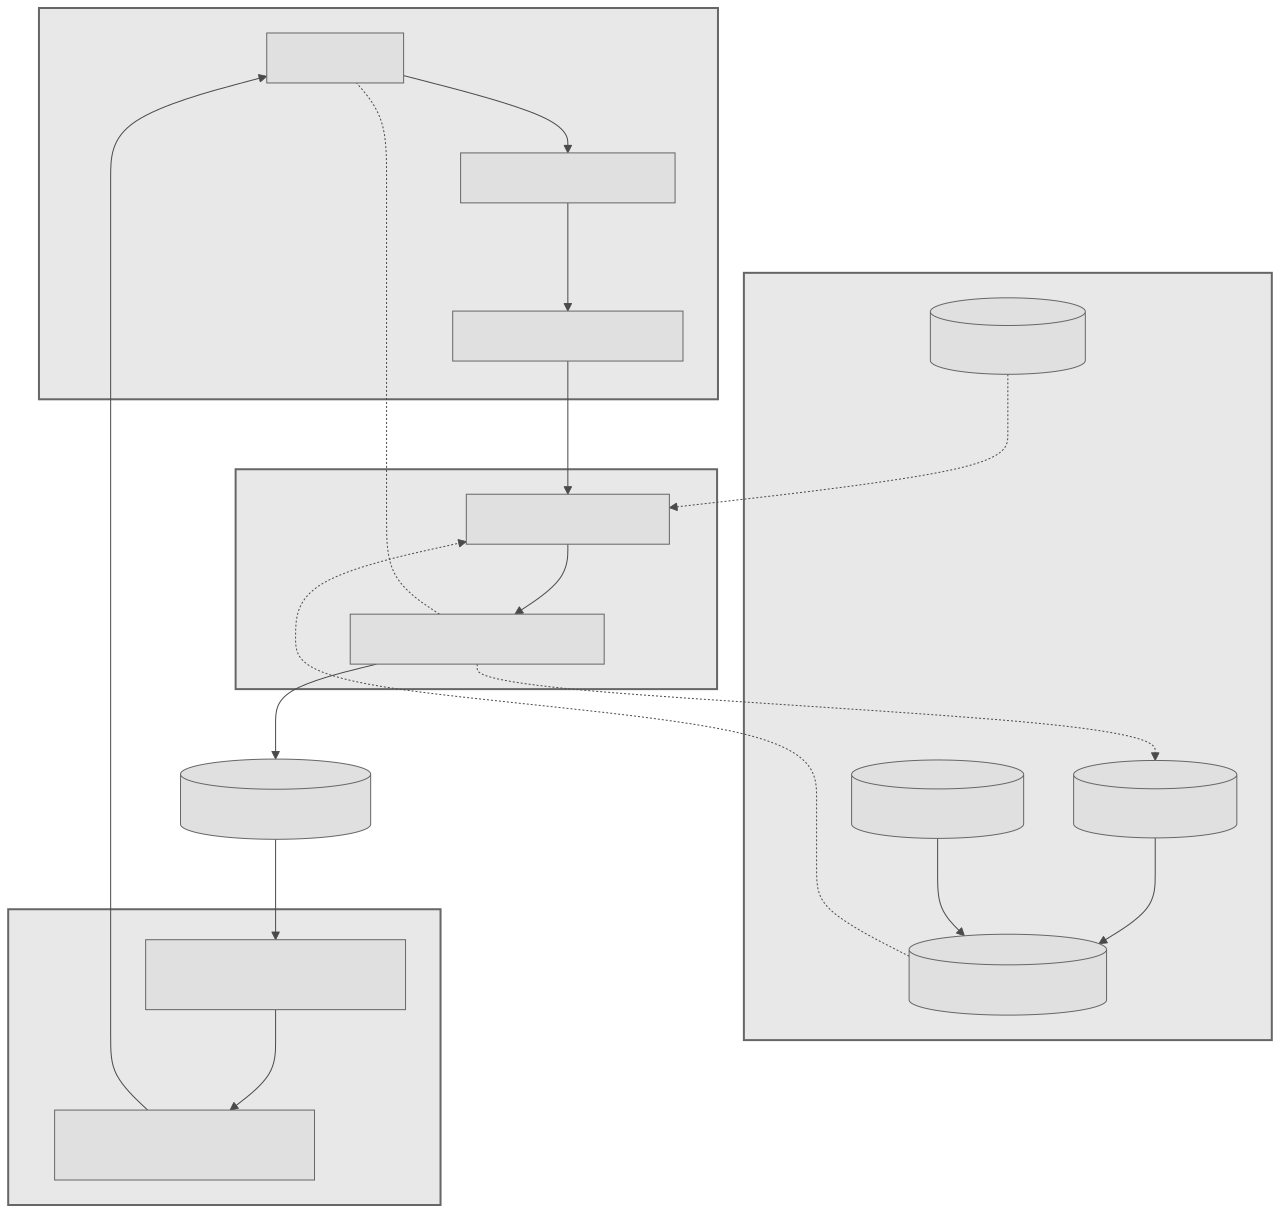
\includegraphics[width=0.95\textwidth,height=\textheight]{figures/architecture.mmd.png}
\caption{Healthcare Analytics Architecture as a Socio-Technical System.
The architecture flows from Clinical Users through a Conversational AI
interface to a healthcare NLP engine for context-aware SQL generation.
Bi-directional arrows represent the iterative `Query \& Refine' loop.
The critical validation step (dotted line) shows domain experts
confirming SQL before results flow to `Organizational Memory' (dashed
line), where they persist independent of staff tenure.}
\end{figure}

The corresponding six step Validated Query Cycle is summarized in Figure
2, which shows how queries move from initial clinical intent through
expert validation into durable organizational memory.

\begin{figure}
\centering
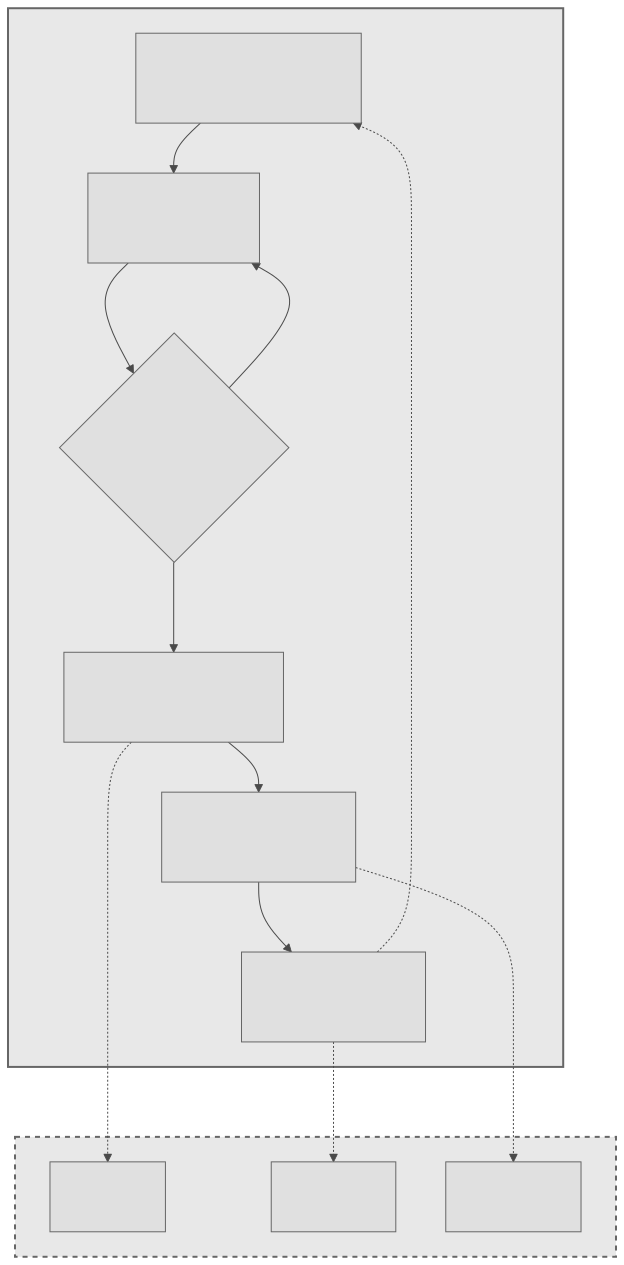
\includegraphics[width=0.8\textwidth,height=\textheight]{figures/knowledge-cycle.mmd.png}
\caption{Six step validated query cycle for Human-in-the-Loop Semantic
Governance. The cycle progresses from Natural Language Intent to
AI-generated SQL, expert review and correction, creation of a Validated
Query Triple, storage in organizational memory, and reuse for future
queries.}
\end{figure}

\subsection{The Process of
Externalization}\label{the-process-of-externalization}

\begin{enumerate}
\def\labelenumi{\arabic{enumi}.}
\tightlist
\item
  \textbf{Query Generation}: A user asks a question. The AI proposes SQL
  based on schema knowledge
  (\citeproc{ref-wang2020}{10},\citeproc{ref-lee2023}{28}).
\item
  \textbf{Semantic Translation}: The AI translates the SQL back into a
  natural language explanation (\citeproc{ref-ziletti2024}{29}).
\item
  \textbf{Expert Validation}: The domain expert confirms or corrects
  this interpretation. \emph{This is the critical moment of
  Externalization.} This ``Human-on-the-Loop'' (HotL) step transforms
  validation into an iterative knowledge capture process
  (\citeproc{ref-bravorocca2023}{19},\citeproc{ref-mosqueirarey2023}{30}).
\item
  \textbf{Artifact Storage}: The validated triple is hashed and stored
  in organizational memory (\citeproc{ref-benbya2004}{31}).
\item
  \textbf{Retrieval}: Future queries semantically match against this
  repository first, retrieving \emph{trusted} human knowledge before
  attempting \emph{probabilistic} generation
  (\citeproc{ref-whittaker2008}{32}).
\end{enumerate}

\section{The Evidence Base: Three
Pillars}\label{the-evidence-base-three-pillars}

The HiL-SG framework is supported by three pillars of empirical evidence
synthesized from over 130 sources.

\subsection{Pillar 1: Analytics Maturity
Evidence}\label{pillar-1-analytics-maturity-evidence}

Healthcare maturity remains chronically low. Assessments reveal only 26
organizations achieved Stage 6 and 13 reached Stage 7 by late 2024
(\citeproc{ref-himss2024}{1},\citeproc{ref-himss2024news}{33}). Most
organizations remain at Stages 0-3, characterized by fragmented data and
limited predictive capabilities (\citeproc{ref-health2020}{34}).
However, maturity is not merely an IT metric; it is a clinical safety
predictor. EMRAM levels 6-7 correlate with 3.25 times higher odds of
better Leapfrog Safety Grades (\citeproc{ref-snowdon2024}{35}). Low
maturity creates a ``low-maturity trap'' where data quality issues (such
as the 39-71\% missing data rates in cancer databases
(\citeproc{ref-yang2021}{36})) remain uncorrected because the experts
who understand the context are leaving.

Critically, low maturity is not simply a status; it is a
self-reinforcing trap. Organizations at Stages 0-3 lack the automated
monitoring and data governance infrastructure needed to detect their own
deficiencies, creating a vicious cycle in which poor data quality goes
unrecognized because no systems exist to measure it. The clinical
consequences of this trap are measurable: one Medicare ACO that
implemented analytics to overcome EHR fragmentation reduced readmission
rates from 24\% to 17.8\% and achieved \$1.6 million in cost savings
(\citeproc{ref-latrella2024}{37}), demonstrating what becomes possible
when organizations escape this cycle. Yet 68\% of healthcare
organizations continue to cite data interoperability as the leading
obstacle to analytics adoption, followed by privacy concerns (64\%) and
insufficient staff training (59\%) (\citeproc{ref-nashid2023}{38}).
Barriers including employee resistance to change and lack of
organizational readiness further stall data-driven initiatives
(\citeproc{ref-shahbaz2019}{39},\citeproc{ref-kamble2019}{40}). The
low-maturity trap thus compounds over time: each year of delayed
investment widens the gap between what the organization could know and
what it actually knows.

\subsection{Pillar 2: Workforce Agility
Evidence}\label{pillar-2-workforce-agility-evidence}

The cost of turnover in informatics is higher than standard IT.
Knowledge loss can cost up to three times annual salary
(\citeproc{ref-massingham2018}{24},\citeproc{ref-oracle2024}{41}). With
30\% of new employees leaving within their first year
(\citeproc{ref-nsi2025}{16}), healthcare IT professionals spend a
limited portion of their employment at full productivity, as specialized
roles require 18-24 months to reach fluency
(\citeproc{ref-ledikwe2013}{13},\citeproc{ref-konrad2022}{21}). This
``revolving door'' prevents the accumulation of the ``Collective
Knowledge Structures'' required for complex task performance
(\citeproc{ref-rao2006}{11}).

The workforce crisis operates at multiple reinforcing levels. At the
strategic level, 53\% of healthcare CIOs have tenures of less than three
years (\citeproc{ref-wittkieffer2024}{5}), producing recurring shifts in
analytics strategy that destabilize long-term initiatives. At the
operational level, 79\% of provider organizations report persistent
shortages in digital health roles
(\citeproc{ref-himssworkforce2024}{6}). At the foundational level, 55\%
of public health informatics specialists intend to leave their positions
(\citeproc{ref-rajamani2025}{7}), draining the specialized talent needed
to maintain analytics infrastructure. This multi-level instability
directly undermines the SECI Socialization mode discussed in the
Theoretical Grounding section: sustained mentorship requires temporal
overlap between experienced practitioners and newcomers, yet the
revolving door at every organizational tier ensures that overlap rarely
materializes. A foundational 2004 study established that healthcare IT
staff had the lowest expected tenure for new hires among all IT sectors
at just 2.9 years (\citeproc{ref-ang2004}{15}). That this two-decade-old
benchmark remains a primary reference point is itself evidence of the
crisis: the field has lacked the stability even to systematically track
its own attrition over the intervening decades.

\subsection{Pillar 3: Technical Enablement
Evidence}\label{pillar-3-technical-enablement-evidence}

NL2SQL has reached a productivity tipping point. Natural language
interfaces report a 63\% increase in self-service adoption and 37\%
reduction in retrieval time (\citeproc{ref-dadi2025}{42}). Precision
medicine platforms achieve 92.5\% accuracy in parsing complex queries
(\citeproc{ref-yang2025}{43}). While current models are ``not yet
sufficiently accurate for unsupervised use''
(\citeproc{ref-ziletti2024}{29}), domain-adapted systems like MedT5SQL
reach 80\% accuracy on benchmarks (\citeproc{ref-marshan2024}{44}).
These tools function as the ``externalization engine'' required for the
HiL-SG framework.

However, NL2SQL is an enabler, not a solution in itself. Its deeper
significance lies in the organizational prerequisites it demands. For an
AI system to translate a natural language question into a correct SQL
query, the organization must first establish validated data models,
explicit business logic definitions, and codified domain terminology
(\citeproc{ref-gal2019}{2},\citeproc{ref-zhang2024}{3}). In other words,
the technology forces organizational discipline as a precondition for
functioning, making it a governance forcing function even before
considering the query results. This reframes NL2SQL from a convenience
tool into a catalyst for the kind of systematic knowledge
externalization that the HiL-SG framework requires. The interface
bridges the semantic gap between clinical experts and technical schema,
allowing non-technical domain experts to interact with data alongside
broader modernization efforts
(\citeproc{ref-anthropic2025}{45}--\citeproc{ref-arora2025}{48}). The
technical barrier thus becomes, paradoxically, a governance opportunity:
the very difficulty of making NL2SQL work correctly compels
organizations to surface and formalize the tacit knowledge that would
otherwise remain trapped in departing experts.

\section{The Analytics Resilience
Index}\label{the-analytics-resilience-index}

To measure success, we propose the \textbf{Analytics Resilience Index
(ARI)}, replacing static checklists with dynamic resilience metrics.

\subsection{Why Resilience, Not
Maturity}\label{why-resilience-not-maturity}

Existing maturity models such as the HIMSS Analytics Maturity Assessment
Model (AMAM) assume linear progression through discrete stages and
implicitly presuppose a stable workforce capable of sustaining each
level once achieved
(\citeproc{ref-himss2024}{1},\citeproc{ref-wang2018}{9}). In practice,
this assumption is violated routinely. An organization that reaches AMAM
Stage 5 but regresses to Stage 3 after the departure of two senior
analysts has not failed to mature; it has failed to be \emph{resilient}.
Static maturity scores capture a snapshot of peak capability but reveal
nothing about the organization's ability to sustain that capability
through disruption. The ARI addresses this gap by shifting the
measurement focus from ``where you are'' to ``how far you fall when
someone leaves.''

\subsection{Operationalizing the ARI}\label{operationalizing-the-ari}

Each ARI dimension (Table 1) can be scored on a Likert-type scale from 1
(fragile) to 5 (antifragile). For example, the ``Knowledge Locus''
dimension would be scored by surveying whether key analytical queries
are documented in a shared, version-controlled repository (score 5) or
known only to named individuals who could leave at any time (score 1).
Similarly, ``Turnover Impact'' could be assessed through scenario
exercises that simulate the departure of a critical team member and
measure the time required to restore reporting capability. An aggregate
ARI score across all dimensions provides a composite indicator of
organizational resilience posture, enabling longitudinal tracking and
cross-institutional benchmarking.

Critically, the ARI complements rather than replaces AMAM. Where AMAM
measures the sophistication of an organization's analytical capabilities
at a point in time, the ARI measures the durability of those
capabilities under workforce stress. An organization should aspire to
high scores on both instruments: AMAM for capability and ARI for
sustainability. Used together, they provide a two-dimensional view of
analytics health that neither instrument offers alone.

\begin{longtable}[]{@{}
  >{\raggedright\arraybackslash}p{(\columnwidth - 6\tabcolsep) * \real{0.2500}}
  >{\raggedright\arraybackslash}p{(\columnwidth - 6\tabcolsep) * \real{0.2500}}
  >{\raggedright\arraybackslash}p{(\columnwidth - 6\tabcolsep) * \real{0.2500}}
  >{\raggedright\arraybackslash}p{(\columnwidth - 6\tabcolsep) * \real{0.2500}}@{}}
\caption{The Analytics Resilience Index (ARI).
\label{tab:ari}}\tabularnewline
\toprule\noalign{}
\begin{minipage}[b]{\linewidth}\raggedright
Dimension
\end{minipage} & \begin{minipage}[b]{\linewidth}\raggedright
Low Resilience (Fragile)
\end{minipage} & \begin{minipage}[b]{\linewidth}\raggedright
High Resilience (Antifragile)
\end{minipage} & \begin{minipage}[b]{\linewidth}\raggedright
Evidence
\end{minipage} \\
\midrule\noalign{}
\endfirsthead
\toprule\noalign{}
\begin{minipage}[b]{\linewidth}\raggedright
Dimension
\end{minipage} & \begin{minipage}[b]{\linewidth}\raggedright
Low Resilience (Fragile)
\end{minipage} & \begin{minipage}[b]{\linewidth}\raggedright
High Resilience (Antifragile)
\end{minipage} & \begin{minipage}[b]{\linewidth}\raggedright
Evidence
\end{minipage} \\
\midrule\noalign{}
\endhead
\bottomrule\noalign{}
\endlastfoot
\textbf{Knowledge Locus} & Knowledge resides in ``Hero'' analysts. &
Knowledge resides in the System/Repository. &
(\citeproc{ref-hong2025}{4},\citeproc{ref-benbya2004}{31}) \\
\textbf{Turnover Impact} & Departure of 1 staff member stops reporting.
& Departure causes minimal disruption; successors inherit queries. &
(\citeproc{ref-rao2006}{11},\citeproc{ref-massingham2018}{24}) \\
\textbf{Validation Mode} & Ad-hoc, email-based, ephemeral. & Systematic,
artifact-based, durable (HiL-SG). &
(\citeproc{ref-moore2018}{27},\citeproc{ref-mosqueirarey2023}{30}) \\
\textbf{Schema Coupling} & Hard-coded reports break on schema change. &
Semantic layer adapts; CI/CD detects drift. &
(\citeproc{ref-mannapur2025}{49},\citeproc{ref-battula2025}{50}) \\
\end{longtable}

\section{The Validator Paradox and Standard
Work}\label{the-validator-paradox-and-standard-work}

A critical objection to HiL-SG is circular: if the framework requires
domain experts to validate AI-generated queries, and the core problem is
that domain experts are leaving, then the framework fails precisely when
it is most needed. This \textbf{Validator Paradox} represents the
strongest counterargument to the approach proposed here, and addressing
it requires moving beyond simplistic reassurance.

The resolution draws on Lean management's concept of ``Standard Work''
(\citeproc{ref-alukal2006}{51}). In this framing, validation is not the
establishment of \emph{eternal truth} but the documentation of the
\emph{current known standard}. Each time an analyst validates a query
triple, they record the best available understanding of how a business
question maps to a data operation at that moment in time. The validation
is time-stamped and contextual, not permanent. Critically, as Alukal and
Manos (\citeproc{ref-alukal2006}{51}) establish, standard work is the
prerequisite for Kaizen (continuous improvement): without a documented
baseline, there is no foundation to improve upon. Each validated query
therefore establishes a floor, not a ceiling. When the next expert
arrives (whether a seasoned veteran or a competent mid-career hire),
they inherit a baseline and can refine it rather than reconstructing
institutional knowledge from scratch.

This mechanism functions as a \textbf{Knowledge Ratchet}
(\citeproc{ref-rao2006}{11}). Each validated triple prevents regression
below the last confirmed state. Even if a subsequent validator is less
experienced than their predecessor, the organization cannot slide below
the previously validated standard. The analogy to version control is
instructive: each commit in a software repository preserves a known-good
state, and future contributors can build upon it even if they
occasionally introduce errors. The ratchet does not guarantee forward
progress, but it does prevent catastrophic backsliding, which is the
central failure mode of institutional amnesia.

Real-world evidence supports this mechanism. UC Davis Health moved from
AMAM Stage 0 to Stage 6 by establishing standardized ``S.M.A.R.T.''
definitions for its analytics metrics
(\citeproc{ref-himss2025ucdavis}{52}). Those codified standards survived
staff turnover precisely because they existed as organizational
artifacts rather than as knowledge held solely by the individuals who
created them. The HiL-SG validated query library serves an analogous
function: it encodes analytical decisions into durable, retrievable
structures that persist independent of any single analyst's tenure.

However, the Validator Paradox is not fully resolved. There exists a
minimum viable expertise threshold below which validation becomes
meaningless. A junior analyst rubber-stamping AI-generated output
without genuine comprehension provides no knowledge ratchet; the
validation artifact exists, but its epistemic value is nil. Identifying
this threshold, and understanding how organizational factors (training,
supervision, query complexity) influence it, remains an open empirical
question. Future work in this series (Paper 2) should measure this
threshold via controlled hallucination injection studies, in which
AI-generated queries containing deliberate errors are presented to
validators of varying experience levels to determine the conditions
under which validation ceases to be meaningful.

\section{Safety as Cognitive Forcing}\label{safety-as-cognitive-forcing}

HiL-SG is fundamentally a \textbf{safety mechanism}, not a productivity
tool. The central risk of unsupervised AI in clinical analytics is what
we term ``laundering hallucinations'': a plausible-sounding but
factually incorrect query result that enters the decision pipeline
undetected and influences clinical or operational choices. Because large
language models generate fluent, confident output regardless of
correctness, the absence of a structured validation step means that
errors arrive dressed in the language of expertise, making them harder
to catch than obviously malformed output.

HiL-SG mitigates this risk through \textbf{Cognitive Forcing Functions}
(\citeproc{ref-ziletti2024}{29}), a design pattern borrowed from
clinical decision-making and safety engineering. By requiring the AI to
explain its reasoning \emph{before} presenting results, the architecture
forces the human validator into System 2 (analytical, deliberate)
thinking rather than allowing System 1 (fast, heuristic) acceptance of
superficially plausible output. User studies confirm the practical
benefit: structured explanation reduces error recovery time by 30 to 40
seconds compared to unstructured output review
(\citeproc{ref-ipeirotis2025}{53}).

The parallel to aviation safety is instructive. Checklists and mandatory
call-outs transformed commercial aviation from a high-risk endeavor into
one of the safest modes of transportation, not by eliminating human
error but by creating procedural structures that surface errors before
they propagate. HiL-SG applies the same principle to analytics: the
mandatory validation step functions as an analytical ``call-out'' that
interrupts the default path of uncritical acceptance. In this framing,
the friction introduced by validation is not a cost; it is the mechanism
of safety itself.

\section{Structural Barriers: Why the Problem
Persists}\label{structural-barriers-why-the-problem-persists}

Failed standardization approaches (e.g., IBM Watson Health
(\citeproc{ref-ibm2022}{54},\citeproc{ref-strickland2019}{55}), Haven
(\citeproc{ref-lavito2021}{56},\citeproc{ref-acchiardo2021}{57}))
demonstrate that centralized models fail clinical reality. Metadata
uncertainties and ``messy'' institution-specific business logic require
localized solutions
(\citeproc{ref-gal2019}{2},\citeproc{ref-yang2020}{58}). HiL-SG
addresses this by capturing \emph{local} logic rather than enforcing
\emph{global} standards.

\section{Limitations}\label{limitations}

This work is a narrative, design science informed framework rather than
a systematic review or multi-site empirical evaluation. The literature
base is concentrated on English-language sources and recent (2024--2025)
workforce and NL2SQL studies, so findings may not capture all regional,
specialty-specific, or technological contexts. The HiL-SG architecture
and the proposed Analytics Resilience Index (ARI) are conceptual
artifacts that require future implementation and validation in diverse
health systems before their effectiveness and generalizability can be
fully established.

\section{Implications and Future
Research}\label{implications-and-future-research}

The crisis of Institutional Amnesia in healthcare requires a structural
shift. As long as analytical maturity is tied to individual tenure,
organizations will remain fragile. By implementing
\textbf{Human-in-the-Loop Semantic Governance}, health systems can
decouple intelligence from turnover, building a library of validated
knowledge that ensures maturity advances even as the workforce evolves.

Future research should empirically validate and refine the HiL-SG
framework and the proposed Analytics Resilience Index. Priority
questions include: how ARI scores correlate with observed continuity of
analytics performance during leadership and staff turnover; whether
HiL-SG mediated natural language to SQL workflows reduce error rates,
recovery time, and rework compared to baseline tooling; and which
governance patterns most effectively balance safety, transparency, and
equity when human validators operate at scale. Prospective multi-site
implementation studies, controlled user experiments, and qualitative
implementation research across diverse health systems will be needed to
test these claims and adapt the framework to varying organizational,
regulatory, and data environments.

\section{Acknowledgments}\label{acknowledgments}

The author (S.T.H.) takes full responsibility for the final content,
conducted the research, and verified all claims and citations. Gemini
CLI (Gemini 3, Google) assisted with manuscript editing and refinement.
Figures were generated using the Mermaid graph language.

\section{Author Contributions}\label{author-contributions}

S.T.H. conceived the research, conducted the literature review, and
wrote the manuscript.

\section{Conflicts of Interest}\label{conflicts-of-interest}

The author declares the following competing interests: Samuel T Harrold
is a contract product advisor at Yuimedi, Inc., which develops
healthcare analytics software including conversational AI platforms
relevant to this review's subject matter. The author is also employed as
a Data Scientist at Indiana University Health. This paper presents an
analytical framework derived from published literature and does not
evaluate or recommend specific commercial products, including those of
the author's affiliated organizations. The views expressed are the
author's own and do not represent the official positions of Indiana
University Health or Yuimedi, Inc.

\section{Data Availability}\label{data-availability}

This is a narrative review synthesizing existing literature. No primary
datasets were generated or analyzed. All data cited are from publicly
available peer-reviewed publications and industry reports, referenced in
the bibliography.

\section{Funding}\label{funding}

Yuimedi provided funding for the author's time writing and researching
this manuscript.

\section{Abbreviations}\label{abbreviations}

AACODS: Authority, Accuracy, Coverage, Objectivity, Date, Significance
AI: Artificial Intelligence AMAM: Analytics Maturity Assessment Model
ARI: Analytics Resilience Index CIO: Chief Information Officer DSR:
Design Science Research EMRAM: Electronic Medical Record Adoption Model
HiL-SG: Human-in-the-Loop Semantic Governance HIMSS: Healthcare
Information Management Systems Society HotL: Human-on-the-Loop IT:
Information Technology NL2SQL: Natural Language to SQL SECI:
Socialization, Externalization, Combination, Internalization SQL:
Structured Query Language

\section{References}\label{references}

\phantomsection\label{refs}
\begin{CSLReferences}{0}{1}
\bibitem[\citeproctext]{ref-himss2024}
\CSLLeftMargin{1. }%
\CSLRightInline{Analytics H. {Analytics maturity assessment model (AMAM)
global report. Healthcare Information and Management Systems Society}
{[}Internet{]}. {HIMSS} Analytics; 2024. Available from:
\url{https://www.himss.org/maturity-models/amam/}}

\bibitem[\citeproctext]{ref-gal2019}
\CSLLeftMargin{2. }%
\CSLRightInline{Gal MS, Rubinfeld DL. {Data Standardization}. NYU Law
Review {[}Internet{]}. 2019;94(4):737--70. Available from:
\url{https://www.nyulawreview.org/issues/volume-94-number-4/data-standardization/}}

\bibitem[\citeproctext]{ref-zhang2024}
\CSLLeftMargin{3. }%
\CSLRightInline{Zhang Y, Callaghan-Koru JA, Koru G. {The challenges and
opportunities of continuous data quality improvement for healthcare
administration data}. JAMIA Open. 2024;7(2):ooae042. }

\bibitem[\citeproctext]{ref-hong2025}
\CSLLeftMargin{4. }%
\CSLRightInline{Hong JH. When does employee turnover matter?
Organizational memory in federal IT. Journal of Public Administration
Research and Theory {[}Internet{]}. 2025; Available from:
\url{https://academic.oup.com/jpart/advance-article-abstract/doi/10.1093/jopart/muaf019/8162522}}

\bibitem[\citeproctext]{ref-wittkieffer2024}
\CSLLeftMargin{5. }%
\CSLRightInline{WittKieffer. {CIO Insights: The State of Healthcare IT
Leadership} {[}Internet{]}. WittKieffer; 2024. Available from:
\url{https://api.wittkieffer.com/wp-content/uploads/2012/10/cio-insights-the-state-of-healthcare-it-leadership-wittkieffer-october-2024.pdf}}

\bibitem[\citeproctext]{ref-himssworkforce2024}
\CSLLeftMargin{6. }%
\CSLRightInline{HIMSS. {The Future of Workforce} {[}Internet{]}.
Healthcare Information; Management Systems Society; 2024. Available
from: \url{https://www.himss.org/resources/the-future-of-workforce/}}

\bibitem[\citeproctext]{ref-rajamani2025}
\CSLLeftMargin{7. }%
\CSLRightInline{Rajamani L S. {Public health informatics specialists in
state and local public health workforce: Insights from public health
workforce interests and needs survey}. Journal of Public Health
Management and Practice {[}Internet{]}. 2025; Available from:
\url{https://academic.oup.com/jpubhealth}}

\bibitem[\citeproctext]{ref-american2023}
\CSLLeftMargin{8. }%
\CSLRightInline{NORC at the University of Chicago AHIMA \&. {Health
information workforce survey report} {[}Internet{]}. American Health
Information Management Association \& {NORC} at the University of
Chicago; 2023. Available from:
\url{https://www.ahima.org/news-publications/press-room-press-releases/2023-press-releases/health-information-workforce-shortages-persist-as-ai-shows-promise-ahima-survey-reveals/}}

\bibitem[\citeproctext]{ref-wang2018}
\CSLLeftMargin{9. }%
\CSLRightInline{Wang K Y., Byrd TA. {Big data analytics: Understanding
its capabilities and potential benefits for healthcare organizations}.
Technological Forecasting and Social Change {[}Internet{]}.
2018;126:3--13. Available from:
\url{https://www.sciencedirect.com/science/article/abs/pii/S0040162516000500}}

\bibitem[\citeproctext]{ref-wang2020}
\CSLLeftMargin{10. }%
\CSLRightInline{Wang S P. {Text-to-SQL generation for question answering
on electronic medical records}. In: Proceedings of the web conference
2020 {[}Internet{]}. 2020. Available from:
\url{https://arxiv.org/abs/1908.01839}}

\bibitem[\citeproctext]{ref-rao2006}
\CSLLeftMargin{11. }%
\CSLRightInline{Rao RD, Argote L. Organizational learning and
forgetting: The effects of turnover and structure. European Management
Review {[}Internet{]}. 2006;3(2):77--85. Available from:
\url{https://onlinelibrary.wiley.com/doi/abs/10.1057/palgrave.emr.1500057}}

\bibitem[\citeproctext]{ref-mayo2016}
\CSLLeftMargin{12. }%
\CSLRightInline{Mayo D C. S. {How can we effect culture change toward
data-driven medicine?} International Journal of Radiation Oncology,
Biology, Physics {[}Internet{]}. 2016; Available from:
\url{https://www.redjournal.org/article/S0360-3016(16)00260-1/fulltext}}

\bibitem[\citeproctext]{ref-ledikwe2013}
\CSLLeftMargin{13. }%
\CSLRightInline{Ledikwe R J. H. {Establishing a health information
workforce: Innovation for low- and middle-income countries}. Human
Resources for Health {[}Internet{]}. 2013; Available from:
\url{https://human-resources-health.biomedcentral.com/articles/10.1186/1478-4491-11-35}}

\bibitem[\citeproctext]{ref-mantas2010}
\CSLLeftMargin{14. }%
\CSLRightInline{Mantas A J. {Recommendations of the International
Medical Informatics Association (IMIA) on education in biomedical and
health informatics: First revision}. Methods of Information in Medicine
{[}Internet{]}. 2010; Available from:
\url{https://pubmed.ncbi.nlm.nih.gov/20054502/}}

\bibitem[\citeproctext]{ref-ang2004}
\CSLLeftMargin{15. }%
\CSLRightInline{Ang \&S S. {Turnover of information technology
professionals: The effects of internal labor market strategies}. {ACM}
{SIGMIS} Database: The {DATABASE} for Advances in Information Systems
{[}Internet{]}. 2004; Available from:
\url{https://dl.acm.org/doi/10.1145/1017114.1017118}}

\bibitem[\citeproctext]{ref-nsi2025}
\CSLLeftMargin{16. }%
\CSLRightInline{NSI Nursing Solutions. {2025 National Health Care
Retention \& RN Staffing Report} {[}Internet{]}. NSI Nursing Solutions;
2024. Available from:
\url{https://www.nsinursingsolutions.com/documents/library/nsi_national_health_care_retention_report.pdf}}

\bibitem[\citeproctext]{ref-tyndall2010}
\CSLLeftMargin{17. }%
\CSLRightInline{Tyndall J. {{AACODS} Checklist. Flinders University}
{[}Internet{]}. 2010. Available from:
\url{https://dspace.flinders.edu.au/jspui/bitstream/2328/3326/4/AACODS_Checklist.pdf}}

\bibitem[\citeproctext]{ref-farnese2019}
\CSLLeftMargin{18. }%
\CSLRightInline{Farnese B M. L. {Managing knowledge in organizations: A
Nonaka's {SECI} model operationalization}. Frontiers in Psychology
{[}Internet{]}. 2019; Available from:
\url{https://www.frontiersin.org/articles/10.3389/fpsyg.2019.02730}}

\bibitem[\citeproctext]{ref-bravorocca2023}
\CSLLeftMargin{19. }%
\CSLRightInline{Bravo Rocca GJ. Human-on-the-loop continual learning
{[}Internet{]} {[}PhD thesis{]}. Universitat Polit{è}cnica de Catalunya;
2023. Available from:
\url{https://www.tdx.cat/bitstream/handle/10803/695722/TGJBR1de1.pdf?sequence=1}}

\bibitem[\citeproctext]{ref-foos2006}
\CSLLeftMargin{20. }%
\CSLRightInline{Foos S T. {Tacit knowledge transfer and the knowledge
disconnect}. Journal of Knowledge Management {[}Internet{]}. 2006;
Available from:
\url{https://www.emerald.com/insight/content/doi/10.1108/13673270610650067/full/html}}

\bibitem[\citeproctext]{ref-konrad2022}
\CSLLeftMargin{21. }%
\CSLRightInline{Konrad \&S I. {Exploring the potential of an {IT}
capability in its bootstrap phase from a task driven onboarding
perspective: Insights toward information infrastructure in healthcare}
{[}Internet{]} {[}Master's thesis{]}. 2022. Available from:
\url{https://www.diva-portal.org/smash/record.jsf?pid=diva2:1684142}}

\bibitem[\citeproctext]{ref-wu2024}
\CSLLeftMargin{22. }%
\CSLRightInline{Wu L F., Li L. {Worldwide prevalence and associated
factors of nursing staff turnover: A systematic review and
meta-analysis}. Nursing Open {[}Internet{]}. 2024;11:e2097. Available
from: \url{https://pmc.ncbi.nlm.nih.gov/articles/PMC10802134/}}

\bibitem[\citeproctext]{ref-ren2024}
\CSLLeftMargin{23. }%
\CSLRightInline{Ren W L. {Global prevalence of nurse turnover rates: A
meta-analysis of 21 studies from 14 countries}. Journal of Nursing
Management {[}Internet{]}. 2024; Available from:
\url{https://pmc.ncbi.nlm.nih.gov/articles/PMC11919231/}}

\bibitem[\citeproctext]{ref-massingham2018}
\CSLLeftMargin{24. }%
\CSLRightInline{Massingham PR. {Measuring the impact of knowledge loss:
A longitudinal study}. Journal of Knowledge Management {[}Internet{]}.
2018; Available from: \url{https://doi.org/10.1108/JKM-08-2016-0338}}

\bibitem[\citeproctext]{ref-zhang2025}
\CSLLeftMargin{25. }%
\CSLRightInline{Zhang D W. {{AI} challenges conventional knowledge
management: Light the way for reframing {SECI} model and Ba theory}.
Journal of Knowledge Management {[}Internet{]}. 2025; Available from:
\url{https://www.emerald.com/insight/content/doi/10.1108/JKM-03-2024-0262/full/html}}

\bibitem[\citeproctext]{ref-goffin2011}
\CSLLeftMargin{26. }%
\CSLRightInline{Goffin \&K K. {Tacit knowledge, lessons learnt, and new
product development}. Journal of Product Innovation Management
{[}Internet{]}. 2011; Available from:
\url{https://onlinelibrary.wiley.com/doi/abs/10.1111/j.1540-5885.2010.00798.x}}

\bibitem[\citeproctext]{ref-moore2018}
\CSLLeftMargin{27. }%
\CSLRightInline{Moore D et al. {ActiveNavigator: Toward real-time
knowledge capture and feedback in active learning spaces}. International
Journal of Engineering Education {[}Internet{]}. 2018;34(2):1--12.
Available from: \url{https://wendyju.com/publications/18_ijee3593.pdf}}

\bibitem[\citeproctext]{ref-lee2023}
\CSLLeftMargin{28. }%
\CSLRightInline{Lee et al G. {EHRSQL: A practical text-to-SQL benchmark
for electronic health records}. In: Proceedings of NeurIPS 2022
{[}Internet{]}. 2023. Available from:
\url{https://arxiv.org/abs/2301.07695}}

\bibitem[\citeproctext]{ref-ziletti2024}
\CSLLeftMargin{29. }%
\CSLRightInline{Ziletti \&D A. {Retrieval augmented text-to-SQL
generation for epidemiological question answering using electronic
health records}. {NAACL} 2024 Clinical {NLP} Workshop {[}Internet{]}.
2024; Available from: \url{https://arxiv.org/abs/2403.09226}}

\bibitem[\citeproctext]{ref-mosqueirarey2023}
\CSLLeftMargin{30. }%
\CSLRightInline{Mosqueira-Rey E et al. Human-in-the-loop machine
learning: A state of the art. Artificial Intelligence Review
{[}Internet{]}. 2023;56:3005--54. Available from:
\url{https://link.springer.com/content/pdf/10.1007/s10462-022-10246-w.pdf}}

\bibitem[\citeproctext]{ref-benbya2004}
\CSLLeftMargin{31. }%
\CSLRightInline{Benbya P H. {Corporate portal: A tool for knowledge
management synchronization}. International Journal of Information
Management {[}Internet{]}. 2004; Available from:
\url{https://doi.org/10.1016/j.ijinfomgt.2003.12.012}}

\bibitem[\citeproctext]{ref-whittaker2008}
\CSLLeftMargin{32. }%
\CSLRightInline{Whittaker S, Hyland P, Wiley M. Design and evaluation of
systems to support interaction capture and retrieval. Personal and
Ubiquitous Computing {[}Internet{]}. 2008;12(3):197--209. Available
from:
\url{https://www.academia.edu/download/41283190/Design_and_evaluation_of_systems_to_supp20160117-25708-98zc50.pdf}}

\bibitem[\citeproctext]{ref-himss2024news}
\CSLLeftMargin{33. }%
\CSLRightInline{Healthcare IT News. {HIMSS launches modernised Analytics
Maturity Assessment Model} {[}Internet{]}. 2024. Available from:
\url{https://www.healthcareitnews.com/news/asia/himss24-apac-adoption-model-analytics-maturity-gets-facelift}}

\bibitem[\citeproctext]{ref-health2020}
\CSLLeftMargin{34. }%
\CSLRightInline{Catalyst H. {The healthcare analytics adoption model: A
roadmap to analytic maturity} {[}Internet{]}. 2020. Available from:
\url{https://www.healthcatalyst.com/learn/insights/healthcare-analytics-adoption-model-roadmap-analytic-maturity}}

\bibitem[\citeproctext]{ref-snowdon2024}
\CSLLeftMargin{35. }%
\CSLRightInline{Snowdon H A., Wright A. {Digital maturity as a predictor
of quality and safety outcomes in {US} hospitals: Cross-sectional
observational study}. Journal of Medical Internet Research
{[}Internet{]}. 2024;26:e56316. Available from:
\url{https://www.jmir.org/2024/1/e56316}}

\bibitem[\citeproctext]{ref-yang2021}
\CSLLeftMargin{36. }%
\CSLRightInline{Yang DX, Khera R, Miccio JA, Jairam V, et al.
{Prevalence of missing data in the national cancer database and
association with overall survival}. JAMA Network Open {[}Internet{]}.
2021;4(3):e211793. Available from:
\url{https://jamanetwork.com/journals/jamanetworkopen/fullarticle/2777777}}

\bibitem[\citeproctext]{ref-latrella2024}
\CSLLeftMargin{37. }%
\CSLRightInline{Latrella \&B M. {Improving patient outcomes while
reducing readmissions with data analytics}. Management in Healthcare
{[}Internet{]}. 2024; Available from:
\url{https://www.ingentaconnect.com/content/hsp/mih/2024/00000008/00000004/art00006}}

\bibitem[\citeproctext]{ref-nashid2023}
\CSLLeftMargin{38. }%
\CSLRightInline{Nashid P S., Hossain MI. {Advanced Business Analytics in
Healthcare: Enhancing Clinical Decision Support and Operational
Efficiency}. Business and Social Sciences {[}Internet{]}.
2023;1(1):1--8. Available from:
\url{https://doi.org/10.25163/business.1110345}}

\bibitem[\citeproctext]{ref-shahbaz2019}
\CSLLeftMargin{39. }%
\CSLRightInline{Shahbaz G M. {Investigating the adoption of big data
analytics in healthcare: The moderating role of resistance to change}.
Journal of Big Data {[}Internet{]}. 2019; Available from:
\url{https://journalofbigdata.springeropen.com/articles/10.1186/s40537-019-0170-y}}

\bibitem[\citeproctext]{ref-kamble2019}
\CSLLeftMargin{40. }%
\CSLRightInline{Kamble G S. S. {A systematic perspective on the
applications of big data analytics in healthcare management}.
International Journal of Healthcare Management {[}Internet{]}. 2019;
Available from:
\url{https://www.tandfonline.com/doi/full/10.1080/20479700.2018.1531606}}

\bibitem[\citeproctext]{ref-oracle2024}
\CSLLeftMargin{41. }%
\CSLRightInline{Oracle. {The real cost of turnover in healthcare}
{[}Internet{]}. 2024. Available from:
\url{https://www.oracle.com/human-capital-management/cost-employee-turnover-healthcare/}}

\bibitem[\citeproctext]{ref-dadi2025}
\CSLLeftMargin{42. }%
\CSLRightInline{Dadi CB, Hoque MR, Ali MM, Ferdausi S, Fatema K, Hasan
MR. {Natural Language Interfaces for Database Management: Bridging the
Gap Between Users and Data through Conversational {AI}}. Journal of
Computer Science and Technology Studies {[}Internet{]}.
2025;7(3):927--33. Available from:
\url{https://al-kindipublisher.com/index.php/jcsts/article/view/9694}}

\bibitem[\citeproctext]{ref-yang2025}
\CSLLeftMargin{43. }%
\CSLRightInline{Yang EW, Waldrup B, et al. {Conversational Artificial
Intelligence for Integrating Social Determinants, Genomics, and Clinical
Data in Precision Medicine: Development and Evaluation}. JMIR
Bioinformatics and Digital Health {[}Internet{]}. 2025; Available from:
\url{https://bioinform.jmir.org/2025/1/e63139}}

\bibitem[\citeproctext]{ref-marshan2024}
\CSLLeftMargin{44. }%
\CSLRightInline{Marshan A A. {MedT5SQL: a transformers-based large
language model for text-to-SQL conversion in the healthcare domain}.
Frontiers in Big Data {[}Internet{]}. 2024; Available from:
\url{https://www.frontiersin.org/articles/10.3389/fdata.2024.1371680}}

\bibitem[\citeproctext]{ref-anthropic2025}
\CSLLeftMargin{45. }%
\CSLRightInline{Anthropic. {Code modernization playbook: A practical
guide to modernizing legacy systems with {AI}} {[}Internet{]}. 2025.
Available from:
\url{https://resources.anthropic.com/code-modernization-playbook}}

\bibitem[\citeproctext]{ref-hendrix1978}
\CSLLeftMargin{46. }%
\CSLRightInline{Hendrix S G. G. {Developing a natural language interface
to complex data}. {ACM} Transactions on Database Systems {[}Internet{]}.
1978; Available from:
\url{https://dl.acm.org/doi/abs/10.1145/320251.320253}}

\bibitem[\citeproctext]{ref-ogunwole2023}
\CSLLeftMargin{47. }%
\CSLRightInline{Ogunwole \&O O. {Modernizing legacy systems: A scalable
approach to next-generation data architectures and seamless
integration}. International Journal of Multidisciplinary Research
{[}Internet{]}. 2023; Available from:
\url{https://www.allmultidisciplinaryjournal.com/uploads/archives/20250306182550_MGE-2025-2-018.1.pdf}}

\bibitem[\citeproctext]{ref-arora2025}
\CSLLeftMargin{48. }%
\CSLRightInline{Arora A. {Challenges of Integrating Artificial
Intelligence in Legacy Systems and Potential Solutions for Seamless
Integration}. {SSRN} {[}Internet{]}. 2025; Available from:
\url{https://papers.ssrn.com/sol3/papers.cfm?abstract_id=5268176}}

\bibitem[\citeproctext]{ref-mannapur2025}
\CSLLeftMargin{49. }%
\CSLRightInline{Mannapur S. Understanding data drift and concept drift
in machine learning systems. International Journal of Scientific
Research {[}Internet{]}. 2025; Available from:
\url{https://www.quantbeckman.com/api/v1/file/5b240742-bf0d-4f8c-a0f9-cb29fab42611.pdf}}

\bibitem[\citeproctext]{ref-battula2025}
\CSLLeftMargin{50. }%
\CSLRightInline{Battula SKY.
\href{https://doi.org/10.63282/3050-9262.IJAIDSML-V6I4P130}{{Adaptive
Data Quality Management for Multi-Cloud Healthcare Warehouses:
FHIR-Aware Semantics and Unsupervised Thresholding}}. International
Journal of Artificial Intelligence, Data Science, and Machine Learning.
2025;6(4):218--26. }

\bibitem[\citeproctext]{ref-alukal2006}
\CSLLeftMargin{51. }%
\CSLRightInline{Alukal VG, Manos A. Lean kaizen: A simplified approach
to process improvement {[}Internet{]}. Milwaukee, WI: ASQ Quality Press;
2006. Available from:
\url{https://books.google.com/books?id=9uqiEAAAQBAJ}}

\bibitem[\citeproctext]{ref-himss2025ucdavis}
\CSLLeftMargin{52. }%
\CSLRightInline{HIMSS. {UC Davis Health: From Stage 0 to AI Heroes}
{[}Internet{]}. Healthcare Information; Management Systems Society;
2025. Available from:
\url{https://pages.himss.org/LP-HA-Case-Study-UC-Davis.html}}

\bibitem[\citeproctext]{ref-ipeirotis2025}
\CSLLeftMargin{53. }%
\CSLRightInline{Ipeirotis \&Z P. {Natural Language Interfaces for
Databases: What Do Users Think?} arXiv preprint arXiv:251114718
{[}Internet{]}. 2025; Available from:
\url{https://arxiv.org/abs/2511.14718}}

\bibitem[\citeproctext]{ref-ibm2022}
\CSLLeftMargin{54. }%
\CSLRightInline{IBM. {Francisco Partners to Acquire IBM's Healthcare
Data and Analytics Assets}. {IBM} Newsroom {[}Internet{]}. 2022;
Available from:
\url{https://newsroom.ibm.com/2022-01-21-Francisco-Partners-to-Acquire-IBMs-Healthcare-Data-and-Analytics-Assets}}

\bibitem[\citeproctext]{ref-strickland2019}
\CSLLeftMargin{55. }%
\CSLRightInline{Strickland E. {IBM Watson, heal thyself: How IBM
overpromised and underdelivered on AI health care}. IEEE Spectrum
{[}Internet{]}. 2019;56(4):24--31. Available from:
\url{https://ieeexplore.ieee.org/abstract/document/8678513/}}

\bibitem[\citeproctext]{ref-lavito2021}
\CSLLeftMargin{56. }%
\CSLRightInline{LaVito A. {Haven, the Amazon-Berkshire-JPMorgan venture
to disrupt healthcare, is disbanding after 3 years}. {CNBC}
{[}Internet{]}. 2021; Available from:
\url{https://www.cnbc.com/2021/01/04/haven-the-amazon-berkshire-jpmorgan-venture-to-disrupt-healthcare-is-disbanding-after-3-years.html}}

\bibitem[\citeproctext]{ref-acchiardo2021}
\CSLLeftMargin{57. }%
\CSLRightInline{Acchiardo JM, Gunderman RB. {The Failure of Haven
Healthcare: Lessons for Radiology Learners}. Academic Radiology
{[}Internet{]}. 2021;28(7):1036--7. Available from:
\url{https://www.academicradiology.org/article/S1076-6332(21)00140-9/abstract}}

\bibitem[\citeproctext]{ref-yang2020}
\CSLLeftMargin{58. }%
\CSLRightInline{Yang J, Chesbrough H, Hurmelinna-Laukkanen P. {The rise,
fall, and resurrection of IBM Watson Health} {[}Internet{]}. University
of Oulu; 2020. Available from:
\url{https://oulurepo.oulu.fi/bitstream/handle/10024/27921/nbnfi-fe2020050424858.pdf}}

\end{CSLReferences}

\end{document}
